

\tikzset{every picture/.style={line width=0.75pt}} %set default line width to 0.75pt        

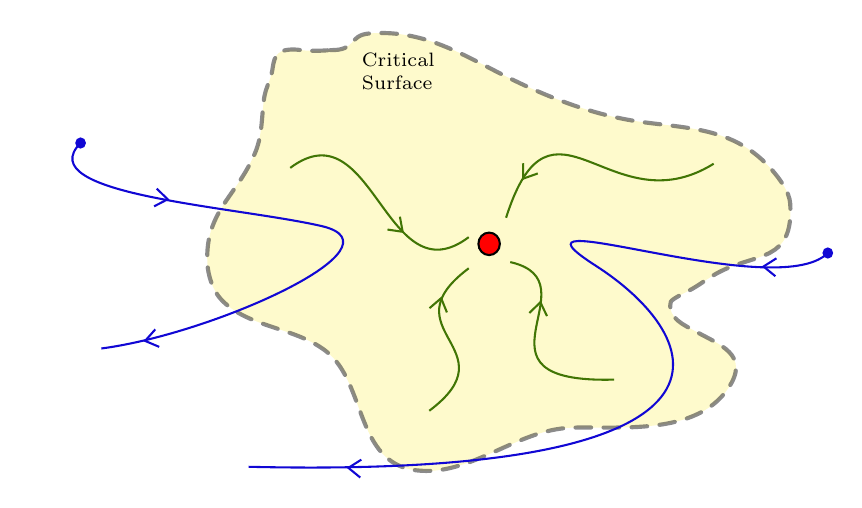
\begin{tikzpicture}[x=0.75pt,y=0.75pt,yscale=-1,xscale=1]
%uncomment if require: \path (0,300); %set diagram left start at 0, and has height of 300

%Curve Lines [id:da7849949621763153] 
\draw [color={rgb, 255:red, 74; green, 74; blue, 74 }  ,draw opacity=0.64 ][fill={rgb, 255:red, 253; green, 242; blue, 133 }  ,fill opacity=0.42 ][line width=1.5] [line join = round][line cap = round] [dash pattern={on 5.63pt off 4.5pt}]  (206.32,43.88) .. controls (219.21,44.16) and (214.87,36.65) .. (225.22,35.85) .. controls (248.43,34.07) and (265.57,43.43) .. (285.33,53.69) .. controls (308.11,65.51) and (331.98,75.35) .. (357.47,78.66) .. controls (381.04,81.72) and (402.12,81.9) .. (419.31,101.85) .. controls (422.66,105.73) and (427.57,112.18) .. (427.9,117.9) .. controls (429.5,146.25) and (412.1,141.26) .. (393.54,150.89) .. controls (389.07,153.22) and (385.04,156.4) .. (380.66,158.92) .. controls (378.85,159.97) and (370.7,163.75) .. (370.36,165.16) .. controls (368.44,173.14) and (377.49,176.66) .. (382.38,179.43) .. controls (393.42,185.69) and (409.22,190.54) .. (397.84,207.08) .. controls (382.08,229.99) and (344.92,224.97) .. (322.26,225.81) .. controls (295.87,226.78) and (273.62,249.57) .. (247.55,246.32) .. controls (218.45,242.69) and (223.5,204.4) .. (204.61,189.24) .. controls (189.75,177.32) and (166.94,177.77) .. (153.94,164.27) .. controls (149.75,159.92) and (147.36,152.58) .. (147.07,146.44) .. controls (145.86,121.29) and (161.59,114.2) .. (170.25,92.93) .. controls (173.76,84.33) and (173.13,75.04) .. (174.55,66.17) .. controls (175.15,62.44) and (177.12,59.06) .. (177.98,55.47) .. controls (179.08,50.93) and (178.49,44.87) .. (184.85,43.88) .. controls (191.93,42.78) and (190.87,45.05) .. (206.32,43.88) -- cycle ;
%Shape: Ellipse [id:dp09682734795909409] 
\draw  [color={rgb, 255:red, 0; green, 0; blue, 0 }  ,draw opacity=1 ][fill={rgb, 255:red, 255; green, 0; blue, 0 }  ,fill opacity=1 ] (277.66,137.21) .. controls (277.66,134.22) and (279.97,131.79) .. (282.83,131.79) .. controls (285.68,131.79) and (288,134.22) .. (288,137.21) .. controls (288,140.21) and (285.68,142.63) .. (282.83,142.63) .. controls (279.97,142.63) and (277.66,140.21) .. (277.66,137.21) -- cycle ;
%Curve Lines [id:da8832046115437673] 
\draw [color={rgb, 255:red, 65; green, 117; blue, 5 }  ,draw opacity=1 ]   (187,100.63) .. controls (227,70.63) and (233,164) .. (273,134) ;
%Curve Lines [id:da948414159458357] 
\draw [color={rgb, 255:red, 65; green, 117; blue, 5 }  ,draw opacity=1 ]   (254,217.63) .. controls (294,187.63) and (233,179) .. (273,149) ;
%Curve Lines [id:da9954148190045367] 
\draw [color={rgb, 255:red, 65; green, 117; blue, 5 }  ,draw opacity=1 ]   (343,202.63) .. controls (267,204.63) and (335,155.63) .. (293,146) ;
%Curve Lines [id:da6038512828805981] 
\draw [color={rgb, 255:red, 65; green, 117; blue, 5 }  ,draw opacity=1 ]   (391,98.63) .. controls (341,129.63) and (313,55.63) .. (291,124.63) ;
%Curve Lines [id:da10801141969503636] 
\draw [color={rgb, 255:red, 17; green, 7; blue, 212 }  ,draw opacity=1 ]   (96,187.63) .. controls (150,180.63) and (244,138.27) .. (202,128.63) .. controls (160,119) and (61,113.63) .. (86,88.63) ;
%Shape: Boxed Bezier Curve [id:dp12977768980803195] 
\draw [color={rgb, 255:red, 17; green, 7; blue, 212 }  ,draw opacity=1 ]   (167,244.63) .. controls (421,250.63) and (387,181.63) .. (334,147.63) .. controls (281,113.63) and (421,166.63) .. (446,141.63) ;
\draw  [color={rgb, 255:red, 17; green, 7; blue, 212 }  ,draw opacity=1 ] (122.67,110.61) -- (127.97,115.76) -- (121.4,119.15) ;
\draw  [color={rgb, 255:red, 17; green, 7; blue, 212 }  ,draw opacity=1 ] (123.88,186.86) -- (117.07,183.98) -- (121.97,178.44) ;
\draw  [color={rgb, 255:red, 17; green, 7; blue, 212 }  ,draw opacity=1 ] (420.74,152.81) -- (415.01,148.14) -- (421.25,144.19) ;
\draw  [color={rgb, 255:red, 17; green, 7; blue, 212 }  ,draw opacity=1 ] (220.74,249.81) -- (215.01,245.14) -- (221.25,241.19) ;
\draw  [color={rgb, 255:red, 65; green, 117; blue, 5 }  ,draw opacity=1 ] (302.22,170.5) -- (307.53,165.36) -- (310.71,172.04) ;
\draw  [color={rgb, 255:red, 65; green, 117; blue, 5 }  ,draw opacity=1 ] (254.1,168.22) -- (259.71,163.4) -- (262.49,170.25) ;
\draw  [color={rgb, 255:red, 65; green, 117; blue, 5 }  ,draw opacity=1 ] (239.84,124.13) -- (241.16,131.4) -- (233.84,130.34) ;
\draw  [color={rgb, 255:red, 65; green, 117; blue, 5 }  ,draw opacity=1 ] (306.26,103.31) -- (299.29,105.78) -- (299.16,98.39) ;
%Shape: Ellipse [id:dp6365405782700908] 
\draw  [draw opacity=0][fill={rgb, 255:red, 17; green, 7; blue, 212 }  ,fill opacity=1 ] (83.41,88.63) .. controls (83.41,87.14) and (84.57,85.92) .. (86,85.92) .. controls (87.43,85.92) and (88.59,87.14) .. (88.59,88.63) .. controls (88.59,90.13) and (87.43,91.34) .. (86,91.34) .. controls (84.57,91.34) and (83.41,90.13) .. (83.41,88.63) -- cycle ;
%Shape: Ellipse [id:dp26949101542259046] 
\draw  [draw opacity=0][fill={rgb, 255:red, 17; green, 7; blue, 212 }  ,fill opacity=1 ] (443.41,141.63) .. controls (443.41,140.14) and (444.57,138.92) .. (446,138.92) .. controls (447.43,138.92) and (448.59,140.14) .. (448.59,141.63) .. controls (448.59,143.13) and (447.43,144.34) .. (446,144.34) .. controls (444.57,144.34) and (443.41,143.13) .. (443.41,141.63) -- cycle ;

% Text Node
\draw (220,44) node [anchor=north west][inner sep=0.75pt]  [font=\scriptsize] [align=left] {Critical \\Surface};


\end{tikzpicture}
